\documentclass[letterpaper,conference]{IEEEtran}
%% CCNC 2013 addition:
%\makeatletter
%\def\ps@headings{%
%	\def\@oddhead{\mbox{}\scriptsize\rightmark \hfil \thepage}%
%	\def\@evenhead{\scriptsize\thepage \hfil \leftmark\mbox{}}%
%	\def\@oddfoot{}%
%	\def\@evenfoot{}}
%\makeatother
%\pagestyle{headings}

\setlength{\textheight}{9.21in}

\ifCLASSINFOpdf
	\usepackage[pdftex]{graphicx}
	\usepackage{epstopdf}
	\graphicspath{{./figures/}}
	\DeclareGraphicsExtensions{.pdf,.jpeg,.png,.eps}
\else
	\usepackage[dvips]{graphicx}
	\graphicspath{{./figures/}}
	\DeclareGraphicsExtensions{.eps}
\fi

\usepackage[cmex10]{amsmath}
\interdisplaylinepenalty=2500
%\usepackage{dblfloatfix}
\usepackage{url}

%\IEEEoverridecommandlockouts

% Title Page
\title{Download and Energy Consumption Optimization Through Localized Cache Exchange}
\author{
%\IEEEauthorblockN{Rachel Kohvakka}
%\IEEEauthorblockA{Department of Computer Science\\
%		Central Michigan University\\
%		Mount Pleasant, MI 48859\\kohva1rm@cmich.edu}
%\and
\IEEEauthorblockN{Troy Johnson}
\IEEEauthorblockA{Department of Computer Science\\
	Central Michigan University\\
	Mount Pleasant, MI 48859\\
	johns4ta@cmich.edu
}
\and
\IEEEauthorblockN{Patrick Seeling\thanks{Please direct correspondence to P. Seeling}}
\IEEEauthorblockA{Department of Computer Science\\
	Central Michigan University\\
	Mount Pleasant, MI 48859\\
	pseeling@ieee.org\footnote{Please direct correspondence to P. Seeling.}}
}

\begin{document}
\maketitle
\pagestyle{empty}
\thispagestyle{empty}
\begin{abstract}
	\boldmath

\end{abstract}

\begin{IEEEkeywords}
%	Mobile applications, Android, connectivity, network traffic
Mobile communication; Middleware; Energy consumption
\end{IEEEkeywords}

\section{Introduction}

\subsection{Scenario Description}

\begin{figure}
	\centering
	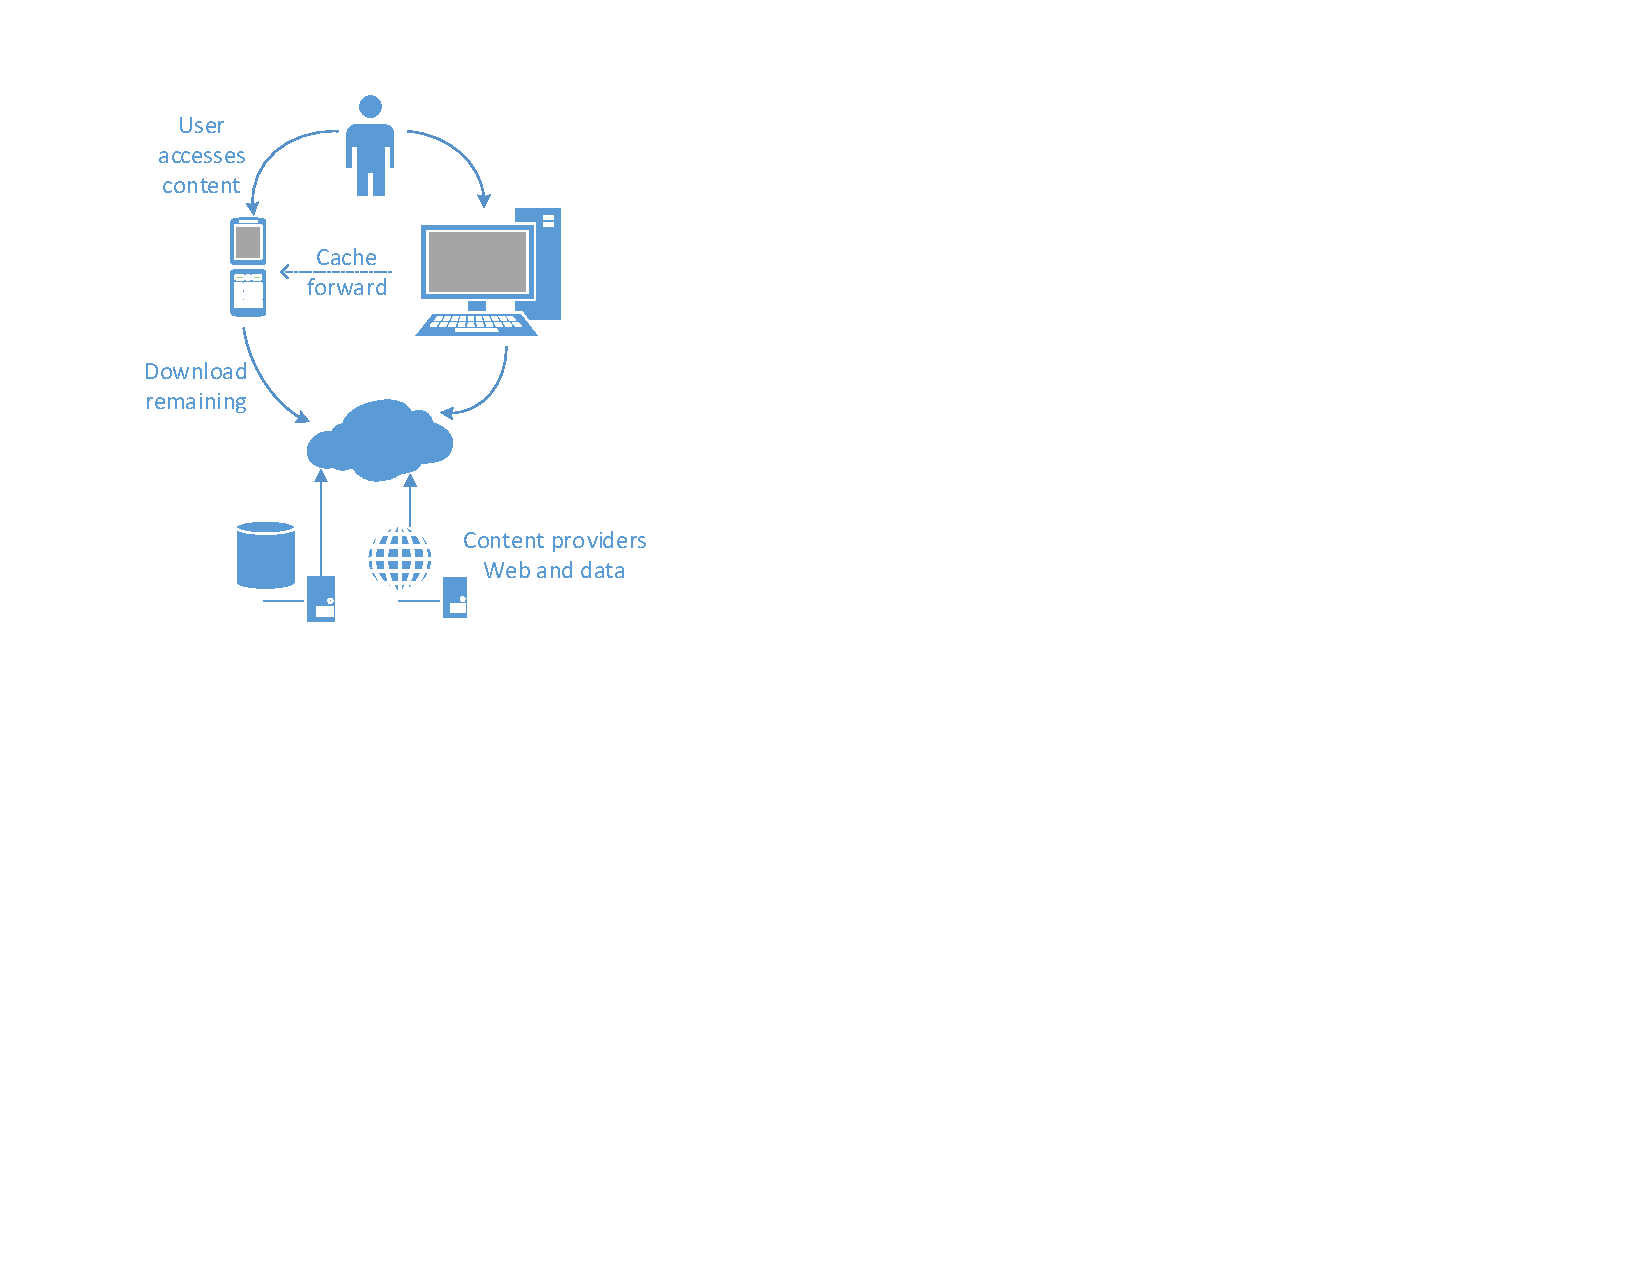
\includegraphics[width=.9\linewidth]{Drawing1}
	\caption{Overall setup of world wide web based content access by a user over time using primary and secondary devices to display the same content. If the devices are able to synchronize their caches through short-range communications, energy savings become possible.}
	\label{fig:setup}
\end{figure}


\section{Methodology and Metrics}
\label{s:setup}
In this section, we outline our setup and evaluation methodology.


\section{Individual Example}
In this section, we outline an individual example for the German news web page for ``Der Spiegel,'' accessible at \url{http://www.spiegel.de} as an example for a rich media and advertising material containing web presence that is frequently updated.
On [insert final date], we performed a speed test online using Internet Explorer as browser instance for a desktop client, Chrome as mobile browser on a Google Nexus 5 instance, and Safari for an iPhone 4 instance provided by \url{WebpageSpeedTest.org} (both mobile clients were traffic shaped to 3G connection emulations).
An example screenshot of the web page as rendered is provided in Figure~\ref{}.
[insert screenshot]

We evaluated the reported data as follows. For each display modality, we gathered the individual web objects requested, and the response sizes and headers for caching information (for response codes 200, as we are not interested in redirects). As in the HTTP specification, the \emph{max-age} directive overrides others, so we initially consider that directive for the cache longevity of the individual objects. If no explicit information is found, we consider the header's \emph{expires} information, which provides a secondary cache lifetime. If both are not found, or if the \emph{expires} date is in the past or right at the request time, we set the cache lifetime we consider here to zero. In case of size differences between the three, we utilize the smallest size as lower boundary.

\subsection{Data Description}
\begin{tabular}{|l|r|r|r|}\hline
Statistic & IE Deskt. & iPhone & Nexus 5\\\hline
& 154 & 132 & 145 \\\hline
& 10402.77	& 8846.39	& 10201.63 \\\hline
& 19103.19	& 13438.05	& 25684.58 \\\hline
& 1.84	&  1.52 &	2.52 \\\hline
\end{tabular}

We initially observe that the desktop version (with Internet Explorer 9 as requesting browser client) exhibits the highest number of objects, followed by the mobile Chrome/Android and Safari mobile/iOS versions, respectively. 
Interestingly, there is only a minor difference in the number of objects between these versions.
Next, we observe that the trend for the average number of bytes is aligned with the number of elements. 
In total, the mobile Chrome version is almost on par with the desktop one (at 92\%) and only the Safari mobile version seeming optimized (at 72\%).
The standard deviation and Coefficient of Variation (CoV) amongst individual element sizes are highest for the mobile Chrome version, indicating more significant size differences than for the safari version, which is one unit lower, while the desktop version falls into the middle.

Next, we evaluate the elements' caching properties on a high level in Table~\ref{tab:scache}. 
\begin{tabular}{|l|r|r|r|}\hline
& 106285.14	& 114780.69	& 114818.28\\\hline
& 125080.27	& 125576.65	& 126090.90\\\hline
& 1.18	& 1.09	& 1.10\\\hline
\end{tabular}
Overall, we note that the highest average caching time is observed for the mobile Chrome access with the Nexus 5 device, trailed immediately by the iOS access and with distance by the desktop browser.
We note that the overall variability in terms of expiration times amongst elements is fairly low and comparable, as indicated by CoV values around 1.1.

\subsection{Evaluation of Local Cache Synchronization}
We now shift the view to the possibility for identical objects to be re-utilized locally to avoid additional download penalties in time and energy consumption.
Simultaneous with a web page request, a local broadcast could ``ask'' for the cached elements for a website to be delivered locally form participating clients. Alternatively, cellular provisioning methods, such as in LTE-A, could initiate the device-to-device local exchange as well.
Once the request is received, the local coordination can take place, which inherently results in the forwarding of elements that are the same across browser instances and which have a future cache lifetime expiration.

We filter out elements that are not similar amongst the different requesting devices, which results in 82 objects with the same URL and size combination. 
While we note an identical cache lifetime for most of these, a slight increase is notable from the Desktop over Safari to Chrome.  Next, we remove items that exhibit a cache lifetime of zero for any of the three requesting clients, resulting in 59 objects, which now exhibit a reduced average cache lifetime for the mobile browsers, whereby mobile Chrome exhibits the shortest.
In turn, we choose the iOS Safari mobile as our exemplary base for calculations.
We illustrate the relative amount of data in the cache in Figure~\ref{} as a function of delayed access time.

[add plot for relative amount of cached data, relative savings]

We observe that a significant amount of the overall data can be cached (and would in turn be suitable for localized sharing).We additionally observe that even for longer durations up to multiple days, significant amounts of data remain in the cache.
Combining the streaming from local clients through either Bluetooth or WLAN technologies, we utilize the approximations outlined in~\cite{} to derive the relative gains of our approach in terms of energy consumption. 
Specifically, we compare our approach (combining locally exchanged caches and cellular downloads of the remainder) with the regular download of all items through the cellular network interface. 






\section{Large Dataset Evaluation}

\section{Conclusion}



\end{document}
